% Track B: full refinement of X25519. A 10-minute talk.
% Build: latexmk -lualatex slides.tex
\documentclass[aspectratio=169,11pt]{beamer}

\usepackage{fontspec}
\setsansfont{DejaVu Sans}
\directlua{
  luaotfload.add_fallback("leanfallback", {"NotoSansMath:mode=harf;", "STIX Two Math:mode=harf;"})
}
\setmonofont{DejaVu Sans Mono}[Scale=0.9, RawFeature={fallback=leanfallback}]

\usepackage{tikz}
\usetikzlibrary{arrows.meta, positioning, calc, fit, backgrounds, shapes.misc, decorations.pathreplacing}

% Colors. Spec side S, impl side I, proof, trusted, gap.
\definecolor{refc}{HTML}{2B6CB0}
\definecolor{realc}{HTML}{C05621}
\definecolor{proofc}{HTML}{2F855A}
\definecolor{trustc}{HTML}{718096}
\definecolor{gapc}{HTML}{C53030}
\definecolor{ink}{HTML}{1A202C}
\definecolor{paper}{HTML}{FFFFFF}

\setbeamercolor{normal text}{fg=ink, bg=paper}
\setbeamercolor{frametitle}{fg=ink}
\setbeamercolor{title}{fg=ink}
\setbeamercolor{structure}{fg=refc}
\setbeamerfont{frametitle}{size=\Large, series=\bfseries}
\setbeamertemplate{navigation symbols}{}
\setbeamertemplate{footline}{%
  \hfill\textcolor{trustc}{\scriptsize\insertframenumber/\inserttotalframenumber}\hspace{1.2em}\vspace{0.8em}}

\tikzset{
  >={Stealth[length=2.4mm]},
  box/.style={draw, rounded corners=3pt, thick, align=center, inner sep=5pt, font=\small},
  ref/.style={box, draw=refc, fill=refc!8},
  real/.style={box, draw=realc, fill=realc!8},
  proof/.style={box, draw=proofc, fill=proofc!10},
  trust/.style={box, draw=trustc, fill=trustc!10},
  gap/.style={box, draw=gapc, fill=gapc!6, dashed},
  tool/.style={box, draw=ink!60, fill=ink!4},
  flow/.style={->, thick, ink!70},
  proved/.style={<->, very thick, proofc},
  label/.style={font=\scriptsize, align=center},
}

\newcommand{\code}[1]{\texttt{#1}}
\newcommand{\refside}[1]{\textcolor{refc}{#1}}
\newcommand{\realside}[1]{\textcolor{realc}{#1}}
% Refinement: S \refines I reads "I refines S". Same macro as the method deck.
\newcommand{\refines}{\sqsubseteq}

\title{Full refinement of X25519}
\subtitle{curve25519-dalek against the hacspec RFC 7748 spec, proved in Lean through Aeneas}
\author{ref-impl-simulation, track B}
\date{November 2026}

\begin{document}

% ---------------------------------------------------------------- 1
\begin{frame}
  \titlepage
  \centering
  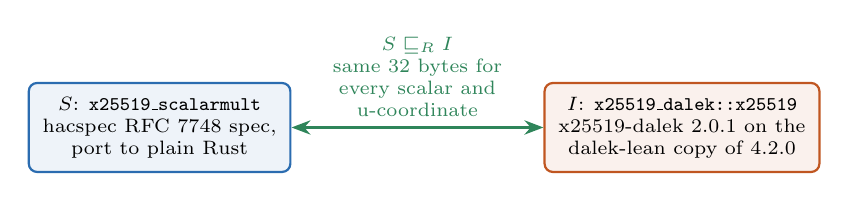
\begin{tikzpicture}
    \node[ref, font=\scriptsize] (r) {$S$: \code{x25519\_scalarmult}\\hacspec RFC 7748 spec,\\port to plain Rust};
    \node[real, font=\scriptsize, right=3.2cm of r] (d) {$I$: \code{x25519\_dalek::x25519}\\x25519-dalek 2.0.1 on the\\dalek-lean copy of 4.2.0};
    \draw[proved] (r) -- node[above, label, text=proofc] {$S \refines_R I$\\same 32 bytes for\\every scalar and\\u-coordinate} (d);
  \end{tikzpicture}
\end{frame}

% ---------------------------------------------------------------- 1b
\begin{frame}{X25519 as an instance of the method}
  The method deck (\code{slides/methodology}) gives the general setup. This deck fills
  in each part for RFC 7748.
  \vspace{1em}

  \centering
  \scriptsize
  \renewcommand{\arraystretch}{1.4}
  \begin{tabular}{l l}
    \textbf{part of the method} & \textbf{X25519} \\
    \hline
    \refside{spec $S$} & hacspec spec of RFC 7748, ported to plain Rust: \code{x25519\_scalarmult} \\
    \realside{impl $I$} & x25519-dalek 2.0.1 and the dalek-lean copy: \code{x25519\_dalek::x25519} \\
    $R_{in}$ & the same scalar and u-coordinate on both sides, no premises \\
    $R_{out}$ & equal 32 bytes \\
    data relation & 5 limbs of 51 bits map to $\mathbb{Z}/p$, limbs below $2^{52}$ \\
    lockstep & the ladder step: 19 field operations \\
    hand-written & one formula (ring identity), the ladder loop (invariant up to a factor) \\
    scope & full refinement: $S \refines_R I$ for \code{x25519\_dalek::x25519} \\
  \end{tabular}
\end{frame}

% ---------------------------------------------------------------- 2
\begin{frame}{The question}
  Two Rust programs compute X25519: the spec $S$ and the impl $I$. Aeneas turns both
  into Lean functions. Can Lean prove $S \refines_R I$?
  \vspace{1.2em}

  \centering
  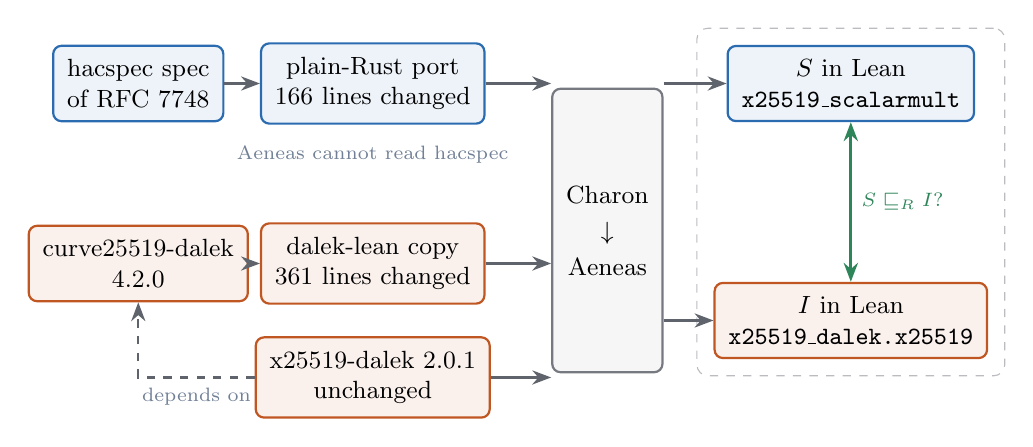
\begin{tikzpicture}[node distance=0.5cm and 0.45cm, every node/.append style={font=\scriptsize}]
    \node[ref] (hs) {hacspec spec\\of RFC 7748};
    \node[ref, right=of hs] (port) {plain-Rust port\\166 lines changed};
    \node[real, below=1.3cm of hs] (up) {curve25519-dalek\\4.2.0};
    \node[real] at (up -| port) (lv) {dalek-lean copy\\361 lines changed};
    \node[real, below=0.4cm of lv] (xd) {x25519-dalek 2.0.1\\unchanged};
    \node[tool, minimum height=3.6cm, anchor=west] (aen) at ($(port.east)!0.5!(xd.east)+(0.8,0)$)
      {Charon\\[2pt]$\downarrow$\\[2pt]Aeneas};
    \node[ref, anchor=west] (lref) at ($(aen.east |- port)+(0.8,0)$) {$S$ in Lean\\\code{x25519\_scalarmult}};
    \coordinate (mid) at ($(lv)!0.5!(xd)$);
    \node[real] (lreal) at (lref |- mid) {$I$ in Lean\\\code{x25519\_dalek.x25519}};

    \draw[flow] (hs) -- (port);
    \draw[flow] (up) -- (lv);
    \draw[flow] (port.east) -- (aen.west |- port.east);
    \draw[flow] (lv.east) -- (aen.west |- lv.east);
    \draw[flow] (xd.east) -- (aen.west |- xd.east);
    \draw[flow, dashed] (xd.west) -| node[pos=0.25, below, label, text=trustc] {depends on} (up.south);
    \draw[flow] (aen.east |- lref) -- (lref);
    \draw[flow] (aen.east |- lreal) -- (lreal);
    \draw[proved] (lref.south) -- node[right, label, text=proofc] {$S \refines_R I$?} (lreal.north);

    \node[label, text=trustc, below=0.15cm of port] {Aeneas cannot read hacspec};
    \begin{scope}[on background layer]
      \node[draw=ink!30, dashed, rounded corners, fit=(lref)(lreal), inner sep=6pt,
            label={[label]above:one Lake project}] {};
    \end{scope}
  \end{tikzpicture}
\end{frame}

% ---------------------------------------------------------------- 3
\begin{frame}[fragile]{What $S \refines_R I$ means here}
  \centering
  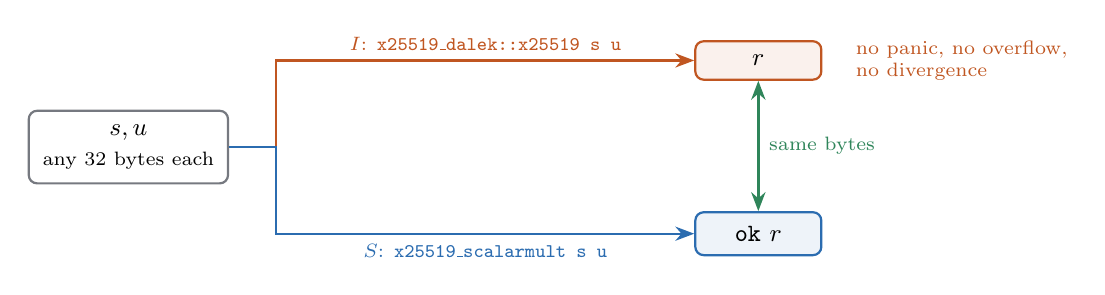
\begin{tikzpicture}
    \node[box, draw=ink!60] (in) at (0,0) {$s, u$\\\scriptsize any 32 bytes each};
    \node[real, minimum width=1.6cm] (rr) at (8, 1.1) {$r$};
    \node[ref, minimum width=1.6cm] (rs) at (8, -1.1) {\code{ok} $r$};
    \draw[flow, realc] (in.east) -- ++(0.6,0) |- node[pos=0.75, above, label, text=realc]
      {$I$: \code{x25519\_dalek::x25519 s u}} (rr.west);
    \draw[flow, refc] (in.east) -- ++(0.6,0) |- node[pos=0.75, below, label, text=refc]
      {$S$: \code{x25519\_scalarmult s u}} (rs.west);
    \draw[proved] (rr) -- node[right, label, text=proofc] {same bytes} (rs);
    \node[label, text=realc, right=0.3cm of rr, align=left]
      {no panic, no overflow,\\no divergence};
  \end{tikzpicture}
  \vspace{1em}

\begin{verbatim}
theorem x25519_refines (k u : Array U8 32#usize) :
    x25519_dalek.x25519.x25519 k u ⦃ r =>
      x25519_ref.x25519_scalarmult k u = ok r ⦄
\end{verbatim}
  \vspace{0.2em}
  \small $R_{in}$: the same inputs. $R_{out}$: the same bytes. No premises. \code{\#print axioms} shows only \code{propext},
  \code{Classical.choice} and \code{Quot.sound}.
\end{frame}

% ---------------------------------------------------------------- 4
\begin{frame}{The proof follows the call path}
  \centering
  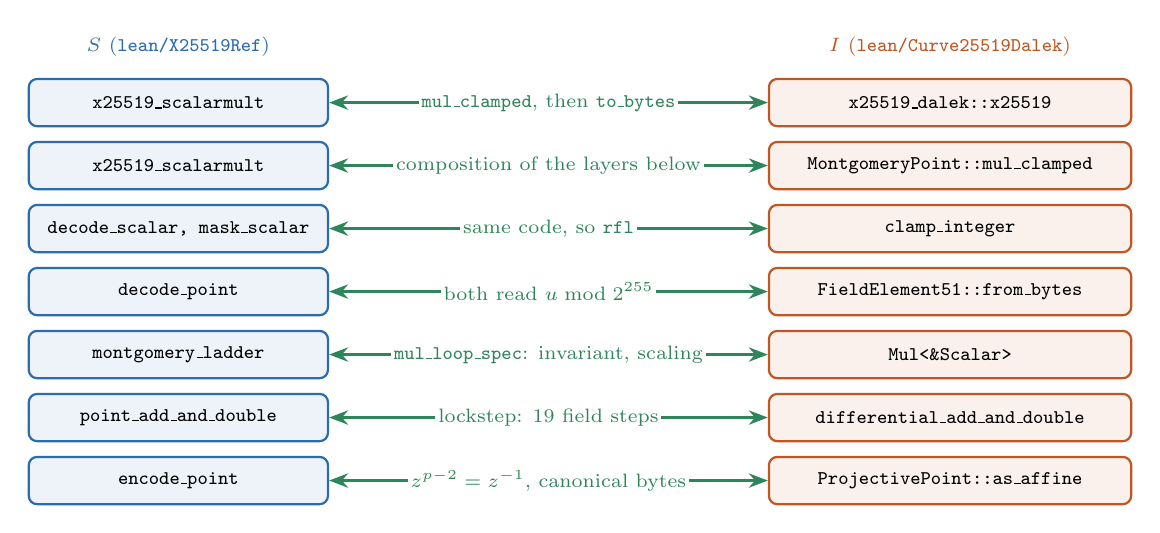
\begin{tikzpicture}[
      lem/.style={label, text=proofc, fill=paper, inner sep=1pt}]
    \foreach \i/\r/\d/\l in {
        0/x25519\_scalarmult/x25519\_dalek::x25519/{\code{mul\_clamped}, then \code{to\_bytes}},
        1/x25519\_scalarmult/MontgomeryPoint::mul\_clamped/{composition of the layers below},
        2/{decode\_scalar, mask\_scalar}/clamp\_integer/{same code, so \code{rfl}},
        3/decode\_point/FieldElement51::from\_bytes/{both read $u \bmod 2^{255}$},
        4/montgomery\_ladder/Mul<\&Scalar>/{\code{mul\_loop\_spec}: invariant, scaling},
        5/point\_add\_and\_double/differential\_add\_and\_double/{lockstep: 19 field steps},
        6/encode\_point/ProjectivePoint::as\_affine/{$z^{p-2} = z^{-1}$, canonical bytes}} {
      \node[ref, minimum width=3.8cm, minimum height=0.6cm, font=\scriptsize\ttfamily] (r\i) at (0, -\i*0.8) {\r};
      \node[real, minimum width=4.6cm, minimum height=0.6cm, font=\scriptsize\ttfamily] (d\i) at (9.8, -\i*0.8) {\d};
      \draw[proved] (r\i) -- node[lem] {\l} (d\i);
    }
    \node[label, text=refc, above=0.15cm of r0] {\textbf{$S$} (\code{lean/X25519Ref})};
    \node[label, text=realc, above=0.15cm of d0] {\textbf{$I$} (\code{lean/Curve25519Dalek})};
  \end{tikzpicture}
  \vspace{0.5em}

  \small Top row: \code{x25519\_refines}, the theorem $S \refines_R I$. Second row: \code{mul\_clamped\_refines}. Each other row is one layer.
\end{frame}

% ---------------------------------------------------------------- 5
\begin{frame}{The ladder step: lockstep on field operations}
  \centering
  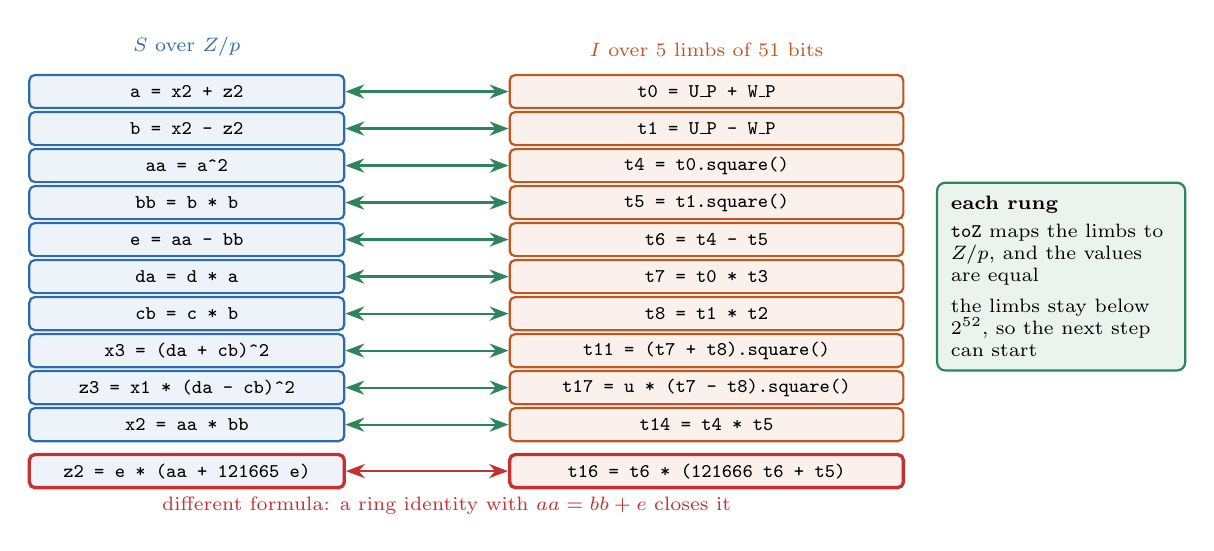
\begin{tikzpicture}[
      op/.style={font=\scriptsize\ttfamily, minimum width=4.0cm, minimum height=0.42cm,
                 inner sep=1.5pt, rounded corners=2pt, thick},
      rop/.style={op, draw=refc, fill=refc!8},
      dop/.style={op, draw=realc, fill=realc!8, minimum width=5.0cm}]
    \foreach \i/\r/\d in {
        0/a = x2 + z2/t0 = U\_P + W\_P,
        1/b = x2 - z2/t1 = U\_P - W\_P,
        2/aa = a\textasciicircum2/t4 = t0.square(),
        3/bb = b * b/t5 = t1.square(),
        4/e = aa - bb/t6 = t4 - t5,
        5/da = d * a/t7 = t0 * t3,
        6/cb = c * b/t8 = t1 * t2,
        7/x3 = (da + cb)\textasciicircum2/t11 = (t7 + t8).square(),
        8/z3 = x1 * (da - cb)\textasciicircum2/t17 = u * (t7 - t8).square(),
        9/x2 = aa * bb/t14 = t4 * t5} {
      \node[rop] (r\i) at (0, -\i*0.47) {\r};
      \node[dop] (d\i) at (6.6, -\i*0.47) {\d};
      \draw[<->, thick, proofc] (r\i) -- (d\i);
    }
    \node[rop, draw=gapc, very thick] (r10) at (0, -10*0.47-0.12) {z2 = e * (aa + 121665 e)};
    \node[dop, draw=gapc, very thick] (d10) at (6.6, -10*0.47-0.12) {t16 = t6 * (121666 t6 + t5)};
    \draw[<->, thick, gapc] (r10) -- (d10);
    \node[label, text=gapc, below=0.2cm of $(r10)!0.5!(d10)$] {different formula: a ring identity with $aa = bb + e$ closes it};
    \node[label, text=refc, above=0.1cm of r0] {\textbf{$S$} over $\mathbb{Z}/p$};
    \node[label, text=realc, above=0.1cm of d0] {\textbf{$I$} over 5 limbs of 51 bits};

    \node[proof, right=0.4cm of d5, text width=2.8cm, font=\scriptsize, align=flush left]
      {\textbf{each rung}\\[2pt]
       \code{toZ} maps the limbs to $\mathbb{Z}/p$, and the values are equal\\[3pt]
       the limbs stay below $2^{52}$, so the next step can start};
  \end{tikzpicture}
\end{frame}

% ---------------------------------------------------------------- 6
\begin{frame}{The ladder: the two loops do not line up}
  \centering
  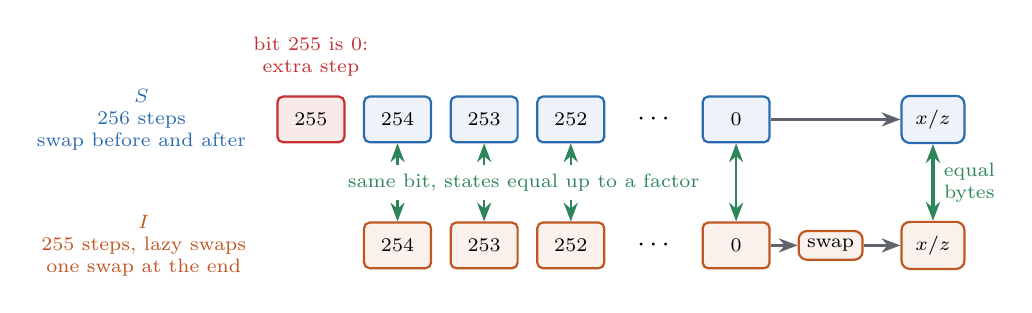
\begin{tikzpicture}[
      it/.style={draw, thick, minimum width=0.85cm, minimum height=0.58cm, font=\scriptsize, rounded corners=2pt},
      rit/.style={it, draw=refc, fill=refc!8},
      dit/.style={it, draw=realc, fill=realc!8}]
    \node[label, text=refc, anchor=east] at (-0.2, 0) {\textbf{$S$}\\256 steps\\swap before and after};
    \node[label, text=realc, anchor=east] at (-0.2, -1.6) {\textbf{$I$}\\255 steps, lazy swaps\\one swap at the end};

    \node[rit, fill=gapc!10, draw=gapc] (r255) at (0.5, 0) {255};
    \foreach \b/\x in {254/1.6, 253/2.7, 252/3.8} {
      \node[rit] (r\b) at (\x, 0) {\b};
      \node[dit] (d\b) at (\x, -1.6) {\b};
      \draw[<->, thick, proofc] (r\b) -- (d\b);
    }
    \node at (4.85, 0) {$\cdots$};
    \node at (4.85, -1.6) {$\cdots$};
    \node[rit] (r0) at (5.9, 0) {0};
    \node[dit] (d0) at (5.9, -1.6) {0};
    \draw[<->, thick, proofc] (r0) -- (d0);
    \node[real, font=\scriptsize, inner sep=3pt] (sw) at (7.1, -1.6) {swap};
    \node[ref, font=\scriptsize] (er) at (8.4, 0) {$x/z$};
    \node[real, font=\scriptsize] (ed) at (8.4, -1.6) {$x/z$};
    \draw[flow] (r0) -- (er);
    \draw[flow] (d0) -- (sw);
    \draw[flow] (sw) -- (ed);
    \draw[proved] (er) -- node[right, label, text=proofc] {equal\\bytes} (ed);

    \node[label, text=gapc, above=0.12cm of r255] {bit 255 is 0:\\extra step};
    \node[label, text=proofc, fill=paper] at (3.2, -0.8) {same bit, states equal up to a factor};
  \end{tikzpicture}
  \vspace{1em}

  \begin{columns}[T]
    \begin{column}{0.45\textwidth}\small
      After the extra step, the state of $S$ is the state of $I$ with the second
      point times $4u$. Each later step scales each point by a nonzero factor.
    \end{column}
    \begin{column}{0.45\textwidth}\small
      The encoding $x/z$ cancels the factor (\code{enc\_ladder\_extra\_step}).
      If $u = 0$, both outputs are 0. This algebra holds over any ring.
    \end{column}
  \end{columns}
\end{frame}

% ---------------------------------------------------------------- 7
\begin{frame}{How this complements dalek-lean}
  \centering
  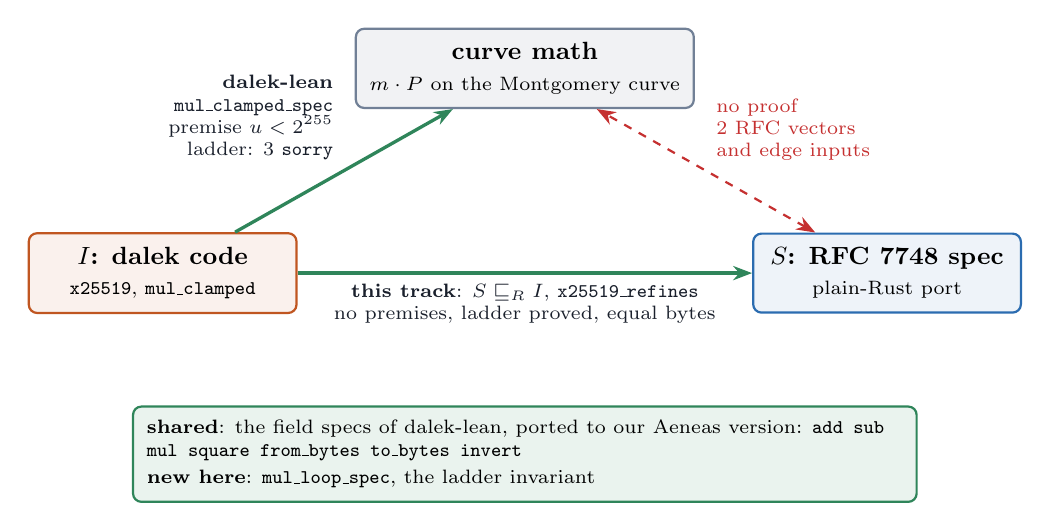
\begin{tikzpicture}
    \node[trust, minimum width=3.4cm] (math) at (0, 2.3)
      {\textbf{curve math}\\\scriptsize $m \cdot P$ on the Montgomery curve};
    \node[real, minimum width=3.4cm] (code) at (-4.6, -0.3)
      {\textbf{$I$: dalek code}\\\scriptsize \code{x25519}, \code{mul\_clamped}};
    \node[ref, minimum width=3.4cm] (refn) at (4.6, -0.3)
      {\textbf{$S$: RFC 7748 spec}\\\scriptsize plain-Rust port};

    \draw[proved, ->] (code) -- node[above left, label, text=ink, align=right]
      {\textbf{dalek-lean}\\\code{mul\_clamped\_spec}\\premise $u < 2^{255}$\\ladder: 3 \code{sorry}} (math);
    \draw[proved, ->] (code) -- node[below, label, text=ink]
      {\textbf{this track}: $S \refines_R I$, \code{x25519\_refines}\\no premises, ladder proved, equal bytes} (refn);
    \draw[gapc, thick, dashed, <->] (refn) -- node[above right, label, text=gapc, align=left]
      {no proof\\2 RFC vectors\\and edge inputs} (math);

    \node[proof, text width=9.6cm, font=\scriptsize, align=flush left] at (0, -2.6)
      {\textbf{shared}: the field specs of dalek-lean, ported to our Aeneas version:
       \code{add sub mul square from\_bytes to\_bytes invert}\\[2pt]
       \textbf{new here}: \code{mul\_loop\_spec}, the ladder invariant};
  \end{tikzpicture}
\end{frame}

% ---------------------------------------------------------------- 8
\begin{frame}{What the theorem trusts}
  \centering
  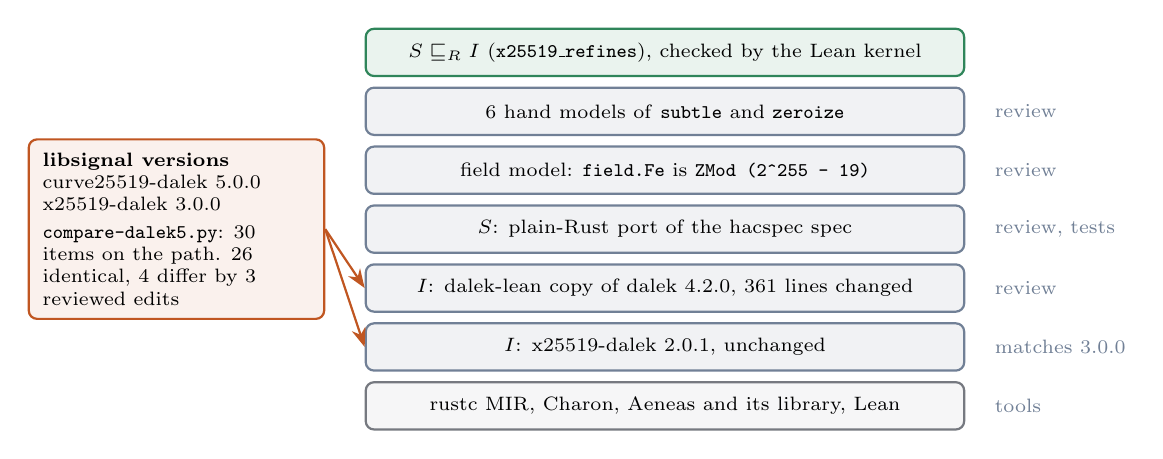
\begin{tikzpicture}[
      layer/.style={box, minimum width=7.6cm, minimum height=0.6cm, font=\scriptsize},
      why/.style={label, text=trustc, anchor=west, align=left}]
    \node[proof, layer] (thm) at (0, 0) {$S \refines_R I$ (\code{x25519\_refines}), checked by the Lean kernel};
    \node[trust, layer, below=0.12cm of thm] (l1) {6 hand models of \code{subtle} and \code{zeroize}};
    \node[trust, layer, below=0.12cm of l1] (l2) {field model: \code{field.Fe} is \code{ZMod (2\textasciicircum255 - 19)}};
    \node[trust, layer, below=0.12cm of l2] (l3) {$S$: plain-Rust port of the hacspec spec};
    \node[trust, layer, below=0.12cm of l3] (l4) {$I$: dalek-lean copy of dalek 4.2.0, 361 lines changed};
    \node[trust, layer, below=0.12cm of l4] (l4b) {$I$: x25519-dalek 2.0.1, unchanged};
    \node[tool, layer, below=0.12cm of l4b] (l5) {rustc MIR, Charon, Aeneas and its library, Lean};

    \foreach \n/\t in {l1/review, l2/review, l3/{review, tests}, l4/review, l4b/{matches 3.0.0}, l5/tools} {
      \node[why] at ([xshift=0.25cm]\n.east) {\t};
    }
    \node[real, text width=3.4cm, font=\scriptsize, align=flush left, left=0.5cm of l3] (d5)
      {\textbf{libsignal versions}\\curve25519-dalek 5.0.0\\x25519-dalek 3.0.0\\[2pt]
       \code{compare-dalek5.py}: 30 items on the path. 26 identical, 4 differ by 3 reviewed edits};
    \draw[flow, realc] (d5.east) -- (l4.west);
    \draw[flow, realc] (d5.east) -- (l4b.west);
  \end{tikzpicture}
  \vspace{0.6em}

  \small Serial u64 backend only. Not \code{fiat}, not \code{curve25519\_dalek\_bits = "32"}.
\end{frame}

% ---------------------------------------------------------------- 9
\begin{frame}{What is not covered, and next steps}
  \centering
  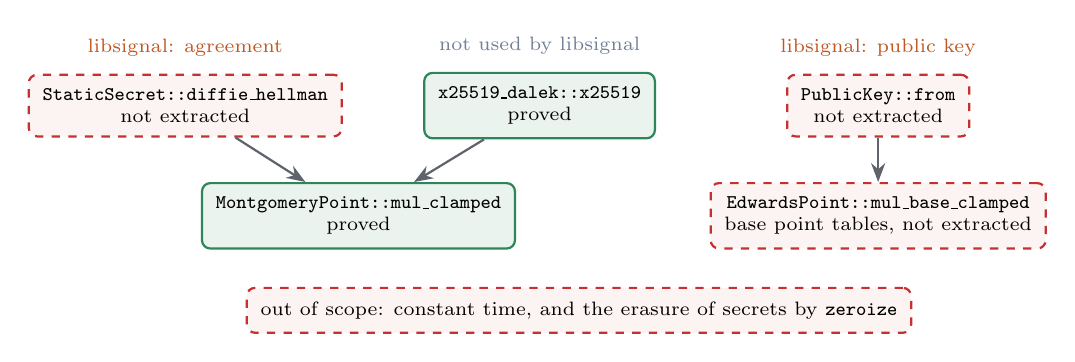
\begin{tikzpicture}[sm/.style={font=\scriptsize}]
    \node[gap, sm] (dh) at (-5.0, 0) {\code{StaticSecret::diffie\_hellman}\\not extracted};
    \node[proof, sm] (xf) at (-0.5, 0) {\code{x25519\_dalek::x25519}\\proved};
    \node[proof, sm] (mc) at (-2.8, -1.4) {\code{MontgomeryPoint::mul\_clamped}\\proved};
    \node[gap, sm] (pk) at (3.8, 0) {\code{PublicKey::from}\\not extracted};
    \node[gap, sm] (mb) at (3.8, -1.4) {\code{EdwardsPoint::mul\_base\_clamped}\\base point tables, not extracted};
    \draw[flow] (dh) -- (mc);
    \draw[flow] (xf) -- (mc);
    \draw[flow] (pk) -- (mb);
    \node[label, text=realc, above=0.1cm of dh] {libsignal: agreement};
    \node[label, text=trustc, above=0.1cm of xf] {not used by libsignal};
    \node[label, text=realc, above=0.1cm of pk] {libsignal: public key};
    \node[gap, sm] at (0, -2.6) {out of scope: constant time, and the erasure of secrets by \code{zeroize}};
  \end{tikzpicture}
  \vspace{0.8em}

  \begin{columns}[T]
    \begin{column}{0.46\textwidth}\footnotesize
      \textbf{Next}\\
      Extract \code{diffie\_hellman}.\\
      Relate $S$ to the curve math.\\
      Build a lockstep tactic for the step.
    \end{column}
    \begin{column}{0.46\textwidth}\footnotesize
      \textbf{Lesson}\\
      Lockstep closes the step.\\
      The ladder needs an invariant by hand.
    \end{column}
  \end{columns}
\end{frame}

\end{document}
